% SPDX-FileCopyrightText: 2026 Jorge Bernal Martínez
%
% SPDX-License-Identifier: CC-BY-4.0

\documentclass[11pt,a4paper]{article}

\usepackage[T1]{fontenc}
\usepackage[utf8]{inputenc}
\usepackage{lmodern}
\usepackage{babel}
\babelprovide[import,main]{spanish}
\usepackage[margin=2.5cm]{geometry}
\usepackage{microtype}
\usepackage{amsmath,amssymb}
\usepackage{graphicx}
\usepackage{booktabs}
\usepackage{xcolor}
\usepackage[numbers,sort&compress]{natbib}
\usepackage{caption}
\usepackage{tikz}
\usetikzlibrary{arrows.meta,positioning,fit,calc,backgrounds}
\usepackage[hidelinks]{hyperref}
\usepackage{cleveref}
\usepackage[section]{placeins}

\addto\captionsspanish{\renewcommand{\tablename}{Tabla}}
\crefname{figure}{figura}{figuras}
\Crefname{figure}{Figura}{Figuras}
\crefname{table}{tabla}{tablas}
\Crefname{table}{Tabla}{Tablas}
\crefname{section}{sección}{secciones}
\Crefname{section}{Sección}{Secciones}
\crefname{subsection}{sección}{secciones}
\Crefname{subsection}{Sección}{Secciones}
\crefname{equation}{ecuación}{ecuaciones}
\Crefname{equation}{Ecuación}{Ecuaciones}
\creflabelformat{equation}{#2(#1)#3}
\newcommand{\crefrangeconjunction}{ a }
\newcommand{\crefpairconjunction}{ y }
\newcommand{\crefmiddleconjunction}{, }
\newcommand{\creflastconjunction}{ y }

\captionsetup{font=small,labelfont=bf}
\graphicspath{{../figures/es/}}
% Generated by bench/make_tables.py: do not edit.
\newcommand{\nAblHistoryOnlyDeformNat}{-6.87}
\newcommand{\nAblHistoryOnlyDeformNatFlicker}{+101}
\newcommand{\nAblHistoryOnlyDeformQ}{-5.20}
\newcommand{\nAblHistoryOnlyDeformQFlicker}{+81}
\newcommand{\nAblHistoryOnlyFastfloorNat}{-2.57}
\newcommand{\nAblHistoryOnlyFastfloorNatFlicker}{+41}
\newcommand{\nAblHistoryOnlyFastfloorQ}{-1.56}
\newcommand{\nAblHistoryOnlyFastfloorQFlicker}{+29}
\newcommand{\nAblHistoryOnlyFloorNat}{-5.28}
\newcommand{\nAblHistoryOnlyFloorNatFlicker}{+77}
\newcommand{\nAblHistoryOnlyFloorQ}{-4.88}
\newcommand{\nAblHistoryOnlyFloorQFlicker}{+73}
\newcommand{\nAblHistoryOnlyNat}{-5.65}
\newcommand{\nAblHistoryOnlyPanNat}{-6.97}
\newcommand{\nAblHistoryOnlyPanNatFlicker}{+105}
\newcommand{\nAblHistoryOnlyPanQ}{-5.32}
\newcommand{\nAblHistoryOnlyPanQFlicker}{+86}
\newcommand{\nAblHistoryOnlyPausestopNat}{-3.37}
\newcommand{\nAblHistoryOnlyPausestopNatFlicker}{+20}
\newcommand{\nAblHistoryOnlyPausestopQ}{-3.27}
\newcommand{\nAblHistoryOnlyPausestopQFlicker}{+11}
\newcommand{\nAblHistoryOnlyQ}{-4.41}
\newcommand{\nAblHistoryOnlyRest}{3.37}
\newcommand{\nAblHistoryOnlyShadowNat}{-1.20}
\newcommand{\nAblHistoryOnlyShadowNatFlicker}{+34}
\newcommand{\nAblHistoryOnlyShadowQ}{-0.80}
\newcommand{\nAblHistoryOnlyShadowQFlicker}{-39}
\newcommand{\nAblHistoryOnlySmokeNat}{-6.46}
\newcommand{\nAblHistoryOnlySmokeNatFlicker}{+91}
\newcommand{\nAblHistoryOnlySmokeQ}{-4.88}
\newcommand{\nAblHistoryOnlySmokeQFlicker}{+69}
\newcommand{\nAblHistoryOnlyStaticNat}{-0.00}
\newcommand{\nAblHistoryOnlyStaticNatFlicker}{-0}
\newcommand{\nAblHistoryOnlyStaticQ}{-0.00}
\newcommand{\nAblHistoryOnlyStaticQFlicker}{+0}
\newcommand{\nAblHistoryOnlyTgtNat}{+50}
\newcommand{\nAblHistoryOnlyTgtNatAbs}{50}
\newcommand{\nAblHistoryOnlyTgtQ}{+31}
\newcommand{\nAblHistoryOnlyTgtQAbs}{31}
\newcommand{\nAblHistoryOnlyWiresNat}{-5.76}
\newcommand{\nAblHistoryOnlyWiresNatFlicker}{+83}
\newcommand{\nAblHistoryOnlyWiresQ}{-4.62}
\newcommand{\nAblHistoryOnlyWiresQFlicker}{+68}
\newcommand{\nAblNoDeformedWindowDeformNat}{-0.59}
\newcommand{\nAblNoDeformedWindowDeformNatFlicker}{+7}
\newcommand{\nAblNoDeformedWindowDeformQ}{-0.72}
\newcommand{\nAblNoDeformedWindowDeformQFlicker}{+11}
\newcommand{\nAblNoDeformedWindowFastfloorNat}{+0.00}
\newcommand{\nAblNoDeformedWindowFastfloorNatFlicker}{+0}
\newcommand{\nAblNoDeformedWindowFastfloorQ}{+0.00}
\newcommand{\nAblNoDeformedWindowFastfloorQFlicker}{+0}
\newcommand{\nAblNoDeformedWindowFloorNat}{+0.00}
\newcommand{\nAblNoDeformedWindowFloorNatFlicker}{+0}
\newcommand{\nAblNoDeformedWindowFloorQ}{+0.00}
\newcommand{\nAblNoDeformedWindowFloorQFlicker}{+0}
\newcommand{\nAblNoDeformedWindowNat}{-0.59}
\newcommand{\nAblNoDeformedWindowPanNat}{+0.00}
\newcommand{\nAblNoDeformedWindowPanNatFlicker}{+0}
\newcommand{\nAblNoDeformedWindowPanQ}{+0.00}
\newcommand{\nAblNoDeformedWindowPanQFlicker}{+0}
\newcommand{\nAblNoDeformedWindowPausestopNat}{+0.00}
\newcommand{\nAblNoDeformedWindowPausestopNatFlicker}{+0}
\newcommand{\nAblNoDeformedWindowPausestopQ}{+0.00}
\newcommand{\nAblNoDeformedWindowPausestopQFlicker}{+0}
\newcommand{\nAblNoDeformedWindowQ}{-0.72}
\newcommand{\nAblNoDeformedWindowRest}{0.00}
\newcommand{\nAblNoDeformedWindowShadowNat}{+0.00}
\newcommand{\nAblNoDeformedWindowShadowNatFlicker}{+0}
\newcommand{\nAblNoDeformedWindowShadowQ}{+0.00}
\newcommand{\nAblNoDeformedWindowShadowQFlicker}{+0}
\newcommand{\nAblNoDeformedWindowSmokeNat}{+0.00}
\newcommand{\nAblNoDeformedWindowSmokeNatFlicker}{+0}
\newcommand{\nAblNoDeformedWindowSmokeQ}{+0.00}
\newcommand{\nAblNoDeformedWindowSmokeQFlicker}{+0}
\newcommand{\nAblNoDeformedWindowStaticNat}{+0.00}
\newcommand{\nAblNoDeformedWindowStaticNatFlicker}{+0}
\newcommand{\nAblNoDeformedWindowStaticQ}{+0.00}
\newcommand{\nAblNoDeformedWindowStaticQFlicker}{+0}
\newcommand{\nAblNoDeformedWindowTgtNat}{+62}
\newcommand{\nAblNoDeformedWindowTgtNatAbs}{62}
\newcommand{\nAblNoDeformedWindowTgtQ}{+104}
\newcommand{\nAblNoDeformedWindowTgtQAbs}{104}
\newcommand{\nAblNoDeformedWindowWiresNat}{+0.00}
\newcommand{\nAblNoDeformedWindowWiresNatFlicker}{+0}
\newcommand{\nAblNoDeformedWindowWiresQ}{+0.00}
\newcommand{\nAblNoDeformedWindowWiresQFlicker}{+0}
\newcommand{\nAblNoLocksDeformNat}{+0.00}
\newcommand{\nAblNoLocksDeformNatFlicker}{+0}
\newcommand{\nAblNoLocksDeformQ}{+0.00}
\newcommand{\nAblNoLocksDeformQFlicker}{+0}
\newcommand{\nAblNoLocksFastfloorNat}{-0.41}
\newcommand{\nAblNoLocksFastfloorNatFlicker}{+1}
\newcommand{\nAblNoLocksFastfloorQ}{-0.09}
\newcommand{\nAblNoLocksFastfloorQFlicker}{+0}
\newcommand{\nAblNoLocksFloorNat}{-0.88}
\newcommand{\nAblNoLocksFloorNatFlicker}{+1}
\newcommand{\nAblNoLocksFloorQ}{-0.38}
\newcommand{\nAblNoLocksFloorQFlicker}{+1}
\newcommand{\nAblNoLocksNat}{-2.56}
\newcommand{\nAblNoLocksPanNat}{+0.00}
\newcommand{\nAblNoLocksPanNatFlicker}{+0}
\newcommand{\nAblNoLocksPanQ}{+0.00}
\newcommand{\nAblNoLocksPanQFlicker}{+0}
\newcommand{\nAblNoLocksPausestopNat}{-4.86}
\newcommand{\nAblNoLocksPausestopNatFlicker}{+64}
\newcommand{\nAblNoLocksPausestopQ}{-5.05}
\newcommand{\nAblNoLocksPausestopQFlicker}{+160}
\newcommand{\nAblNoLocksQ}{-2.88}
\newcommand{\nAblNoLocksRest}{0.00}
\newcommand{\nAblNoLocksShadowNat}{+0.00}
\newcommand{\nAblNoLocksShadowNatFlicker}{+0}
\newcommand{\nAblNoLocksShadowQ}{+0.00}
\newcommand{\nAblNoLocksShadowQFlicker}{+0}
\newcommand{\nAblNoLocksSmokeNat}{+0.00}
\newcommand{\nAblNoLocksSmokeNatFlicker}{+0}
\newcommand{\nAblNoLocksSmokeQ}{+0.00}
\newcommand{\nAblNoLocksSmokeQFlicker}{+0}
\newcommand{\nAblNoLocksStaticNat}{-4.11}
\newcommand{\nAblNoLocksStaticNatFlicker}{+118}
\newcommand{\nAblNoLocksStaticQ}{-6.01}
\newcommand{\nAblNoLocksStaticQFlicker}{+360}
\newcommand{\nAblNoLocksTgtNat}{+25}
\newcommand{\nAblNoLocksTgtNatAbs}{25}
\newcommand{\nAblNoLocksTgtQ}{+3}
\newcommand{\nAblNoLocksTgtQAbs}{3}
\newcommand{\nAblNoLocksWiresNat}{+0.00}
\newcommand{\nAblNoLocksWiresNatFlicker}{+0}
\newcommand{\nAblNoLocksWiresQ}{+0.00}
\newcommand{\nAblNoLocksWiresQFlicker}{+0}
\newcommand{\nAblNoMissingFillDeformNat}{-0.16}
\newcommand{\nAblNoMissingFillDeformNatFlicker}{+2}
\newcommand{\nAblNoMissingFillDeformQ}{-0.11}
\newcommand{\nAblNoMissingFillDeformQFlicker}{+2}
\newcommand{\nAblNoMissingFillFastfloorNat}{-0.38}
\newcommand{\nAblNoMissingFillFastfloorNatFlicker}{+2}
\newcommand{\nAblNoMissingFillFastfloorQ}{-0.41}
\newcommand{\nAblNoMissingFillFastfloorQFlicker}{+4}
\newcommand{\nAblNoMissingFillFloorNat}{-0.35}
\newcommand{\nAblNoMissingFillFloorNatFlicker}{+3}
\newcommand{\nAblNoMissingFillFloorQ}{-0.45}
\newcommand{\nAblNoMissingFillFloorQFlicker}{+5}
\newcommand{\nAblNoMissingFillNat}{-0.35}
\newcommand{\nAblNoMissingFillPanNat}{-0.19}
\newcommand{\nAblNoMissingFillPanNatFlicker}{+2}
\newcommand{\nAblNoMissingFillPanQ}{-0.14}
\newcommand{\nAblNoMissingFillPanQFlicker}{+2}
\newcommand{\nAblNoMissingFillPausestopNat}{+0.00}
\newcommand{\nAblNoMissingFillPausestopNatFlicker}{+0}
\newcommand{\nAblNoMissingFillPausestopQ}{-0.00}
\newcommand{\nAblNoMissingFillPausestopQFlicker}{+0}
\newcommand{\nAblNoMissingFillQ}{-0.37}
\newcommand{\nAblNoMissingFillRest}{0.01}
\newcommand{\nAblNoMissingFillShadowNat}{+0.00}
\newcommand{\nAblNoMissingFillShadowNatFlicker}{+0}
\newcommand{\nAblNoMissingFillShadowQ}{+0.00}
\newcommand{\nAblNoMissingFillShadowQFlicker}{+0}
\newcommand{\nAblNoMissingFillSmokeNat}{-0.01}
\newcommand{\nAblNoMissingFillSmokeNatFlicker}{+0}
\newcommand{\nAblNoMissingFillSmokeQ}{-0.01}
\newcommand{\nAblNoMissingFillSmokeQFlicker}{+0}
\newcommand{\nAblNoMissingFillStaticNat}{+0.00}
\newcommand{\nAblNoMissingFillStaticNatFlicker}{+0}
\newcommand{\nAblNoMissingFillStaticQ}{+0.00}
\newcommand{\nAblNoMissingFillStaticQFlicker}{+0}
\newcommand{\nAblNoMissingFillTgtNat}{+27}
\newcommand{\nAblNoMissingFillTgtNatAbs}{27}
\newcommand{\nAblNoMissingFillTgtQ}{+25}
\newcommand{\nAblNoMissingFillTgtQAbs}{25}
\newcommand{\nAblNoMissingFillWiresNat}{-0.65}
\newcommand{\nAblNoMissingFillWiresNatFlicker}{+4}
\newcommand{\nAblNoMissingFillWiresQ}{-0.74}
\newcommand{\nAblNoMissingFillWiresQFlicker}{+8}
\newcommand{\nAblNoReactiveNat}{-2.27}
\newcommand{\nAblNoReactiveQ}{-1.44}
\newcommand{\nAblNoReactiveRest}{0.00}
\newcommand{\nAblNoReactiveSmokeNat}{-2.27}
\newcommand{\nAblNoReactiveSmokeNatFlicker}{+4}
\newcommand{\nAblNoReactiveSmokeQ}{-1.44}
\newcommand{\nAblNoReactiveSmokeQFlicker}{+1}
\newcommand{\nAblNoReactiveTgtNat}{+133}
\newcommand{\nAblNoReactiveTgtNatAbs}{133}
\newcommand{\nAblNoReactiveTgtQ}{+140}
\newcommand{\nAblNoReactiveTgtQAbs}{140}
\newcommand{\nAblNoThinFrontDeformNat}{+0.00}
\newcommand{\nAblNoThinFrontDeformNatFlicker}{+0}
\newcommand{\nAblNoThinFrontDeformQ}{+0.00}
\newcommand{\nAblNoThinFrontDeformQFlicker}{+0}
\newcommand{\nAblNoThinFrontFastfloorNat}{+0.00}
\newcommand{\nAblNoThinFrontFastfloorNatFlicker}{+0}
\newcommand{\nAblNoThinFrontFastfloorQ}{+0.00}
\newcommand{\nAblNoThinFrontFastfloorQFlicker}{+0}
\newcommand{\nAblNoThinFrontFloorNat}{+0.00}
\newcommand{\nAblNoThinFrontFloorNatFlicker}{+0}
\newcommand{\nAblNoThinFrontFloorQ}{+0.00}
\newcommand{\nAblNoThinFrontFloorQFlicker}{+0}
\newcommand{\nAblNoThinFrontNat}{-0.22}
\newcommand{\nAblNoThinFrontPanNat}{+0.00}
\newcommand{\nAblNoThinFrontPanNatFlicker}{+0}
\newcommand{\nAblNoThinFrontPanQ}{+0.00}
\newcommand{\nAblNoThinFrontPanQFlicker}{+0}
\newcommand{\nAblNoThinFrontPausestopNat}{+0.00}
\newcommand{\nAblNoThinFrontPausestopNatFlicker}{-0}
\newcommand{\nAblNoThinFrontPausestopQ}{+0.00}
\newcommand{\nAblNoThinFrontPausestopQFlicker}{-0}
\newcommand{\nAblNoThinFrontQ}{-0.16}
\newcommand{\nAblNoThinFrontRest}{0.00}
\newcommand{\nAblNoThinFrontShadowNat}{+0.00}
\newcommand{\nAblNoThinFrontShadowNatFlicker}{+0}
\newcommand{\nAblNoThinFrontShadowQ}{+0.00}
\newcommand{\nAblNoThinFrontShadowQFlicker}{+0}
\newcommand{\nAblNoThinFrontSmokeNat}{-0.00}
\newcommand{\nAblNoThinFrontSmokeNatFlicker}{-0}
\newcommand{\nAblNoThinFrontSmokeQ}{-0.00}
\newcommand{\nAblNoThinFrontSmokeQFlicker}{+0}
\newcommand{\nAblNoThinFrontStaticNat}{+0.00}
\newcommand{\nAblNoThinFrontStaticNatFlicker}{+0}
\newcommand{\nAblNoThinFrontStaticQ}{+0.00}
\newcommand{\nAblNoThinFrontStaticQFlicker}{+0}
\newcommand{\nAblNoThinFrontTgtNat}{+12}
\newcommand{\nAblNoThinFrontTgtNatAbs}{12}
\newcommand{\nAblNoThinFrontTgtQ}{+12}
\newcommand{\nAblNoThinFrontTgtQAbs}{12}
\newcommand{\nAblNoThinFrontWiresNat}{-0.22}
\newcommand{\nAblNoThinFrontWiresNatFlicker}{+3}
\newcommand{\nAblNoThinFrontWiresQ}{-0.16}
\newcommand{\nAblNoThinFrontWiresQFlicker}{+0}
\newcommand{\nAblWindowOnlyDeformNat}{+0.00}
\newcommand{\nAblWindowOnlyDeformNatFlicker}{+0}
\newcommand{\nAblWindowOnlyDeformQ}{+0.00}
\newcommand{\nAblWindowOnlyDeformQFlicker}{+0}
\newcommand{\nAblWindowOnlyFastfloorNat}{+0.02}
\newcommand{\nAblWindowOnlyFastfloorNatFlicker}{-0}
\newcommand{\nAblWindowOnlyFastfloorQ}{+0.00}
\newcommand{\nAblWindowOnlyFastfloorQFlicker}{+0}
\newcommand{\nAblWindowOnlyFloorNat}{+0.03}
\newcommand{\nAblWindowOnlyFloorNatFlicker}{-1}
\newcommand{\nAblWindowOnlyFloorQ}{-0.01}
\newcommand{\nAblWindowOnlyFloorQFlicker}{-0}
\newcommand{\nAblWindowOnlyNat}{-0.30}
\newcommand{\nAblWindowOnlyPanNat}{+0.00}
\newcommand{\nAblWindowOnlyPanNatFlicker}{+0}
\newcommand{\nAblWindowOnlyPanQ}{+0.00}
\newcommand{\nAblWindowOnlyPanQFlicker}{+0}
\newcommand{\nAblWindowOnlyPausestopNat}{+0.38}
\newcommand{\nAblWindowOnlyPausestopNatFlicker}{+58}
\newcommand{\nAblWindowOnlyPausestopQ}{+0.33}
\newcommand{\nAblWindowOnlyPausestopQFlicker}{+38}
\newcommand{\nAblWindowOnlyQ}{-0.03}
\newcommand{\nAblWindowOnlyRest}{0.03}
\newcommand{\nAblWindowOnlyShadowNat}{+0.00}
\newcommand{\nAblWindowOnlyShadowNatFlicker}{+0}
\newcommand{\nAblWindowOnlyShadowQ}{+0.00}
\newcommand{\nAblWindowOnlyShadowQFlicker}{+0}
\newcommand{\nAblWindowOnlySmokeNat}{+0.00}
\newcommand{\nAblWindowOnlySmokeNatFlicker}{+0}
\newcommand{\nAblWindowOnlySmokeQ}{+0.00}
\newcommand{\nAblWindowOnlySmokeQFlicker}{+0}
\newcommand{\nAblWindowOnlyStaticNat}{-0.97}
\newcommand{\nAblWindowOnlyStaticNatFlicker}{+161}
\newcommand{\nAblWindowOnlyStaticQ}{-0.39}
\newcommand{\nAblWindowOnlyStaticQFlicker}{+147}
\newcommand{\nAblWindowOnlyTgtNat}{+161}
\newcommand{\nAblWindowOnlyTgtNatAbs}{161}
\newcommand{\nAblWindowOnlyTgtQ}{+147}
\newcommand{\nAblWindowOnlyTgtQAbs}{147}
\newcommand{\nAblWindowOnlyWiresNat}{+0.00}
\newcommand{\nAblWindowOnlyWiresNatFlicker}{+0}
\newcommand{\nAblWindowOnlyWiresQ}{+0.00}
\newcommand{\nAblWindowOnlyWiresQFlicker}{+0}
\newcommand{\nFlickerB}{11.1}
\newcommand{\nFlickerNat}{7.1}
\newcommand{\nFlickerNoAA}{24.3}
\newcommand{\nFlickerP}{12.0}
\newcommand{\nFlickerQ}{9.8}
\newcommand{\nFlickerTAAg}{12.8}
\newcommand{\nFlickerTAApt}{11.9}
\newcommand{\nFlickerUQ}{8.8}
\newcommand{\nFlipB}{0.0398}
\newcommand{\nFlipNat}{0.0236}
\newcommand{\nFlipNoAA}{0.0467}
\newcommand{\nFlipP}{0.0419}
\newcommand{\nFlipQ}{0.0340}
\newcommand{\nFlipTAAg}{0.0409}
\newcommand{\nFlipTAApt}{0.0487}
\newcommand{\nFlipUQ}{0.0309}
\newcommand{\nGainAllB}{1.78}
\newcommand{\nGainAllNat}{5.75}
\newcommand{\nGainAllP}{1.00}
\newcommand{\nGainAllQ}{2.84}
\newcommand{\nGainAllUQ}{3.92}
\newcommand{\nGainMotionB}{1.53}
\newcommand{\nGainMotionNat}{5.85}
\newcommand{\nGainMotionP}{0.69}
\newcommand{\nGainMotionQ}{2.82}
\newcommand{\nGainMotionUQ}{3.87}
\newcommand{\nGhostCutNat}{49}
\newcommand{\nGhostCutP}{49}
\newcommand{\nGhostCutQ}{47}
\newcommand{\nGhostHistNatOne}{23.0}
\newcommand{\nGhostHistPOne}{34.0}
\newcommand{\nGhostHistQOne}{28.2}
\newcommand{\nGhostHwNatOne}{18.1}
\newcommand{\nGhostHwPOne}{30.7}
\newcommand{\nGhostHwQOne}{26.6}
\newcommand{\nGhostNoFillNatOne}{35.3}
\newcommand{\nGhostNoFillPOne}{59.9}
\newcommand{\nGhostNoFillQOne}{49.8}
\newcommand{\nGhostTaaNatOne}{32.2}
\newcommand{\nGhostVsHistNat}{44}
\newcommand{\nGhostVsHistP}{29}
\newcommand{\nGhostVsHistQ}{35}
\newcommand{\nHistShareB}{29}
\newcommand{\nHistShareNat}{47}
\newcommand{\nHistShareP}{33}
\newcommand{\nHistShareQ}{29}
\newcommand{\nHistShareUQ}{29}
\newcommand{\nMemBHd}{127}
\newcommand{\nMemBQhd}{226}
\newcommand{\nMemBUhd}{508}
\newcommand{\nMemNatHd}{189}
\newcommand{\nMemNatQhd}{335}
\newcommand{\nMemNatUhd}{755}
\newcommand{\nMemPHd}{95}
\newcommand{\nMemPQhd}{169}
\newcommand{\nMemPUhd}{379}
\newcommand{\nMemQHd}{151}
\newcommand{\nMemQQhd}{269}
\newcommand{\nMemQUhd}{605}
\newcommand{\nMemUQHd}{188}
\newcommand{\nMemUQQhd}{333}
\newcommand{\nMemUQUhd}{750}
\newcommand{\nMsMovingBHd}{2.0}
\newcommand{\nMsMovingBQhd}{3.6}
\newcommand{\nMsMovingBUhd}{8.0}
\newcommand{\nMsMovingNatHd}{1.4}
\newcommand{\nMsMovingNatQhd}{2.5}
\newcommand{\nMsMovingNatUhd}{5.5}
\newcommand{\nMsMovingPHd}{1.8}
\newcommand{\nMsMovingPQhd}{3.1}
\newcommand{\nMsMovingPUhd}{7.0}
\newcommand{\nMsMovingQHd}{2.0}
\newcommand{\nMsMovingQQhd}{3.6}
\newcommand{\nMsMovingQUhd}{8.1}
\newcommand{\nMsMovingUQHd}{2.0}
\newcommand{\nMsMovingUQQhd}{3.6}
\newcommand{\nMsMovingUQUhd}{8.2}
\newcommand{\nMsPerFrameHd}{0.12}
\newcommand{\nMsPerFrameUhd}{0.48}
\newcommand{\nMsStillBHd}{0.6}
\newcommand{\nMsStillBQhd}{1.1}
\newcommand{\nMsStillBUhd}{2.5}
\newcommand{\nMsStillNatHd}{0.8}
\newcommand{\nMsStillNatQhd}{1.4}
\newcommand{\nMsStillNatUhd}{3.2}
\newcommand{\nMsStillPHd}{0.6}
\newcommand{\nMsStillPQhd}{1.1}
\newcommand{\nMsStillPUhd}{2.4}
\newcommand{\nMsStillQHd}{0.6}
\newcommand{\nMsStillQQhd}{1.1}
\newcommand{\nMsStillQUhd}{2.6}
\newcommand{\nMsStillUQHd}{0.7}
\newcommand{\nMsStillUQQhd}{1.2}
\newcommand{\nMsStillUQUhd}{2.6}
\newcommand{\nNumScenes}{13}
\newcommand{\nPsnrAllB}{31.85}
\newcommand{\nPsnrAllBestTAA}{30.06}
\newcommand{\nPsnrAllNat}{35.81}
\newcommand{\nPsnrAllNoAA}{27.62}
\newcommand{\nPsnrAllP}{31.07}
\newcommand{\nPsnrAllQ}{32.90}
\newcommand{\nPsnrAllTAAg}{29.45}
\newcommand{\nPsnrAllTAApt}{30.04}
\newcommand{\nPsnrAllUQ}{33.98}
\newcommand{\nPsnrMotionB}{31.25}
\newcommand{\nPsnrMotionNat}{35.56}
\newcommand{\nPsnrMotionNoAA}{27.14}
\newcommand{\nPsnrMotionP}{30.40}
\newcommand{\nPsnrMotionQ}{32.54}
\newcommand{\nPsnrMotionTAAg}{29.38}
\newcommand{\nPsnrMotionTAApt}{29.68}
\newcommand{\nPsnrMotionUQ}{33.58}
\newcommand{\nWinsB}{12}
\newcommand{\nWinsNat}{13}
\newcommand{\nWinsP}{10}
\newcommand{\nWinsQ}{13}
\newcommand{\nWinsUQ}{13}
\newcommand{\nWorstGainB}{-0.14}
\newcommand{\nWorstGainNat}{3.99}
\newcommand{\nWorstGainP}{-1.10}
\newcommand{\nWorstGainQ}{0.70}
\newcommand{\nWorstGainUQ}{1.57}
\newcommand{\nWorstSceneB}{fast floor}
\newcommand{\nWorstSceneEsB}{suelo r\'apido}
\newcommand{\nWorstSceneEsNat}{suelo r\'apido}
\newcommand{\nWorstSceneEsP}{suelo r\'apido}
\newcommand{\nWorstSceneEsQ}{suelo r\'apido}
\newcommand{\nWorstSceneEsUQ}{suelo r\'apido}
\newcommand{\nWorstSceneNat}{fast floor}
\newcommand{\nWorstSceneP}{fast floor}
\newcommand{\nWorstSceneQ}{fast floor}
\newcommand{\nWorstSceneUQ}{fast floor}

\newcommand{\FLIP}{\reflectbox{F}LIP}
\newcommand{\vect}[1]{\mathbf{#1}}

\title{Antialiasing temporal híbrido con ventana:\\reconstrucción de los píxeles en movimiento a partir de un anillo de muestras con jitter}
\author{Jorge Bernal Martínez\\
  \small Desarrollador del motor de juegos UPBGE\\
  \small\texttt{jbernalmartinez@gmail.com}}
\date{Noviembre de 2026\\[4pt]\footnotesize \copyright{} 2026 Jorge Bernal Martínez. \\ Esta obra está bajo la licencia Creative Commons Atribución 4.0 Internacional (CC BY 4.0).}

\begin{document}
\maketitle

\begin{abstract}
El antialiasing temporal (TAA), y los escaladores temporales construidos sobre él, acumulan un historial recursivo que se remuestrea en cada fotograma en que el píxel se mueve. El remuestreo repetido emborrona el contenido en movimiento, y el acotado de color por vecindad que limita el ghosting también borra los detalles finos. Presentamos el \emph{antialiasing temporal híbrido con ventana} (HWTAA, \emph{Hybrid Windowed Temporal Antialiasing}). HWTAA guarda las muestras con jitter de los últimos $N$ fotogramas, sin procesar, en un búfer en anillo compacto de 8 bytes por muestra, y reconstruye cada píxel en movimiento directamente a partir de ellas: cada muestra pasada se lleva al fotograma actual una sola vez y de forma exacta, mediante una matriz cerrada por fotograma, se pondera por su distancia al centro del píxel y se acepta por la identidad del objeto en lugar de por un acotado de color. Los píxeles en reposo conservan un historial recursivo, que converge más allá de la ventana, cuesta menos y parpadea menos; los dos estimadores se mezclan por píxel según su movimiento. Un relleno del peso ausente restaura las superficies que descubren los objetos en movimiento, una máscara reactiva trata las superficies transparentes y unos bloqueos de luma mantienen los detalles finos en el historial. En \nNumScenes{} escenas sintéticas, renderizadas con los shaders de producción y comparadas con una referencia de 36 muestras, HWTAA a resolución nativa mejora el PSNR de un TAA de calidad de producción en \nGainAllNat{}\,dB de media y en \nWinsNat{} de \nNumScenes{} escenas; su modo de escalado Calidad, que renderiza el 44\,\% de los píxeles, lo sigue mejorando en \nGainAllQ{}\,dB, en \nWinsQ{} de \nNumScenes{}. El resolve cabe en 64 registros. Su coste estimado a 1080p en una GPU de la clase GTX~1060 es de \nMsStillQHd{}\,ms para los píxeles en reposo y de \nMsMovingQHd{}\,ms con toda la pantalla en movimiento (modo Calidad). HWTAA forma parte del renderizador eevee-game del motor de juegos UPBGE.
\end{abstract}

\section{Introducción}

Los renderizadores en tiempo real toman una muestra por píxel y por fotograma y confían al tiempo el resto. El antialiasing temporal~\cite{karis2014taa,salvi2016taa,yang2020survey} desplaza la proyección una fracción de píxel en cada fotograma (jitter), reproyecta al fotograma actual un historial acumulado mediante vectores de movimiento, descarta las partes que ya no pertenecen al píxel, normalmente acotándolo al rango de color de la vecindad $3\times3$ actual, y mezcla el fotograma actual con un peso pequeño. Escaladores temporales como FSR~2 y 3~\cite{amd2023fsr2,amd2024fsr3}, DLSS~\cite{liu2020dlss} o el supermuestreo neuronal~\cite{xiao2020neural} extienden la misma recursión a resoluciones de render inferiores a la de salida.

La recursión es un filtro de respuesta al impulso infinita (IIR) y tiene dos debilidades conocidas. Primera: el historial se remuestrea en cada fotograma en que el píxel se mueve. Todo filtro de remuestreo atenúa las frecuencias próximas al límite de Nyquist del píxel; aplicado una vez por fotograma, la atenuación se acumula y el contenido en movimiento acaba emborronado. Yang et al.~\cite{yang2009amortized} analizaron este efecto y lo limitaron con búferes de historial subpíxel y un factor de mezcla adaptativo; el TAA de producción lo reduce con filtros más nítidos como Catmull-Rom~\cite{catmull1974splines,jimenez2016filmic}. Segunda: el acotado de color no distingue un detalle fino submuestreado de uno desocluido. Un cable de una décima de píxel de ancho falta en la mayoría de las vecindades actuales, así que el acotado borra lo que el historial había acumulado, y el resultado parpadea.

Observamos que la información que necesita el TAA ya se calcula en cada fotograma: son las propias muestras con jitter. Un historial es un resumen con pérdidas de ellas, cómodo porque cuesta una textura por fotograma. Si en su lugar se guardan las muestras sin procesar de una ventana corta de fotogramas, un píxel en movimiento puede reconstruirse directamente a partir de ellas. Cada muestra pasada se lleva entonces al fotograma actual una sola vez, a partir de su propia profundidad y de las transformaciones de cámara y de objeto de ambos fotogramas, de modo que nunca se remuestrea una imagen intermedia. La visibilidad puede decidirse por la identidad de la superficie a la que pertenece cada muestra, que es exacta, en lugar de por estadísticas de color, que no lo son. Este es un estimador de respuesta al impulso finita (FIR). Su debilidad es la inversa de la del historial: su soporte es de $N$ fotogramas, así que un píxel en reposo no converge más allá de $N$ muestras, mientras que un historial converge indefinidamente y cuesta unas pocas lecturas.

HWTAA combina ambos. Los píxeles en movimiento usan la ventana, los píxeles en reposo usan el historial, y la salida los mezcla según el movimiento del píxel. Nuestras contribuciones son:
\begin{itemize}
\item Un estimador temporal híbrido FIR/IIR, elegido por píxel según su movimiento, en el que la ventana elimina el emborronado por remuestreo del contenido en movimiento y el historial conserva la convergencia, la estabilidad y el bajo coste del TAA para el contenido en reposo (\cref{sec:overview}).
\item Un anillo de muestras que guarda, por texel de render y fotograma, la clave de objeto, la profundidad inversa, las marcas de estabilidad y de transparencia, el color y la luma mediana en 8 bytes (\cref{sec:ring}).
\item Una reproyección cerrada por muestra: una matriz $4\times4$ por fotograma pasado lleva un texel de render y su profundidad inversa directamente al espacio de pesos del píxel de salida, de modo que una muestra cuesta tres multiplicaciones-sumas, una división y una lectura de memoria compartida (\cref{sec:window}).
\item Visibilidad por identidad sin acotado de color, un relleno del peso ausente para las superficies desocluidas y un descarte de fotogramas por luma mediana para el sombreado que se mueve por su cuenta (\cref{sec:window,sec:missing,sec:reactive}).
\item Una evaluación en \nNumScenes{} escenas que ejecuta los shaders GLSL de producción, con PSNR, \FLIP{}~\cite{andersson2020flip}, SSIM~\cite{wang2004ssim} y una métrica de parpadeo, ablaciones de cada componente y un modelo de coste y memoria contrastado con las cifras publicadas por AMD para FSR (\cref{sec:evaluation}).
\end{itemize}

\section{Trabajo relacionado}

\paragraph{Antialiasing espacial.} Los filtros morfológicos como FXAA~\cite{lottes2009fxaa} y SMAA~\cite{jimenez2012smaa} detectan bordes en la imagen final y mezclan a través de ellos. Son baratos y estables, pero no pueden recuperar el detalle que la única muestra por píxel no captó, que es el caso de los detalles finos y la textura subpíxel.

\paragraph{Reproyección y supermuestreo amortizado.} La caché de reproyección inversa~\cite{nehab2007reprojection} reutiliza el sombreado del fotograma anterior proyectando en él el píxel actual. El supermuestreo amortizado~\cite{yang2009amortized} acumula muestras con jitter de forma recursiva, analiza el emborronado que causa remuestrear el historial y lo reduce con varios búferes subpíxel. El sobremuestreo espacio-temporal~\cite{herzog2010upsampling} combina un filtro temporal recursivo con un filtro espacial bilateral conjunto. Scherzer et al.~\cite{scherzer2012coherence} recopilan estos métodos. Todos ellos mantienen un historial recursivo; HWTAA también lo mantiene, para los píxeles en reposo, y lo sustituye para los píxeles en movimiento.

\paragraph{Antialiasing y escalado temporal en videojuegos.} El TAA de los videojuegos~\cite{karis2014taa,jimenez2016filmic} reproyecta un historial con vectores de movimiento, lo muestrea con un filtro nítido y lo acota o recorta a la vecindad actual; el recorte por varianza~\cite{salvi2016taa} ajusta la caja de recorte a la media y la desviación típica de la vecindad. Yang et al.~\cite{yang2020survey} recopilan la familia y sus artefactos: emborronado, ghosting, parpadeo y pérdida de detalles finos. El TAA adaptativo~\cite{marrs2018ataa} traza rayos en los píxeles donde falla el historial. FSR~2~\cite{amd2023fsr2} añade detección de desoclusión por profundidad, una máscara reactiva para superficies transparentes y \emph{bloqueos} (locks) que protegen los detalles finos del acotado; el historial de HWTAA usa bloqueos con el mismo fin y con otra detección y otra vida (\cref{sec:history}). Los escaladores aprendidos~\cite{liu2020dlss,xiao2020neural} sustituyen el descarte diseñado a mano por una red, pero siguen alimentándola con un historial deformado. Poudel et al.~\cite{poudel2026wavelet} separan la salida de un escalador neuronal en bandas de frecuencia; aquí se usa una separación del historial en una banda baja que se recorta y una banda alta que se conserva, para los píxeles en reposo al escalar.

\paragraph{Renderizado sin fotogramas y búferes de muestras profundos.} El renderizado sin fotogramas (frameless)~\cite{bishop1994frameless} actualiza las muestras de forma asíncrona y muestra lo que contenga el búfer; la caché de render~\cite{walter1999rendercache} reproyecta muestras individuales trazadas por rayos a nuevas vistas como puntos. El renderizado sin fotogramas adaptativo~\cite{dayal2005frameless} es el trabajo previo más cercano: guarda las muestras recientes de un trazador de rayos sin fotogramas en un \emph{búfer temporalmente profundo} y reconstruye cada imagen mostrada con filtros espacio-temporales cuya extensión se adapta al cambio espacial y temporal local. HWTAA se diferencia en tres aspectos. Cada muestra pasada se lleva al fotograma actual con geometría exacta, lo que elimina el movimiento del filtro en lugar de estrecharlo. La visibilidad se decide por la identidad del objeto. Y la ventana es la mitad de un híbrido con un historial recursivo, con un coste fijo por fotograma dentro de una canalización de rasterización. No conocemos ningún TAA ni escalador temporal en tiempo real que reconstruya los píxeles en movimiento a partir de una ventana de muestras pasadas sin procesar reproyectadas individualmente.

\paragraph{Eliminación de ruido.} El filtrado espacio-temporal guiado por varianza~\cite{schied2017svgf} y sus sucesores también acumulan un historial validado por profundidad, normales e identidad de objeto. Nuestra prueba de identidad es de la misma naturaleza; la diferencia vuelve a ser que la ventana no acumula.

\section{Método}
\label{sec:method}

\subsection{Visión general}
\label{sec:overview}

\begin{figure}[t]
\centering
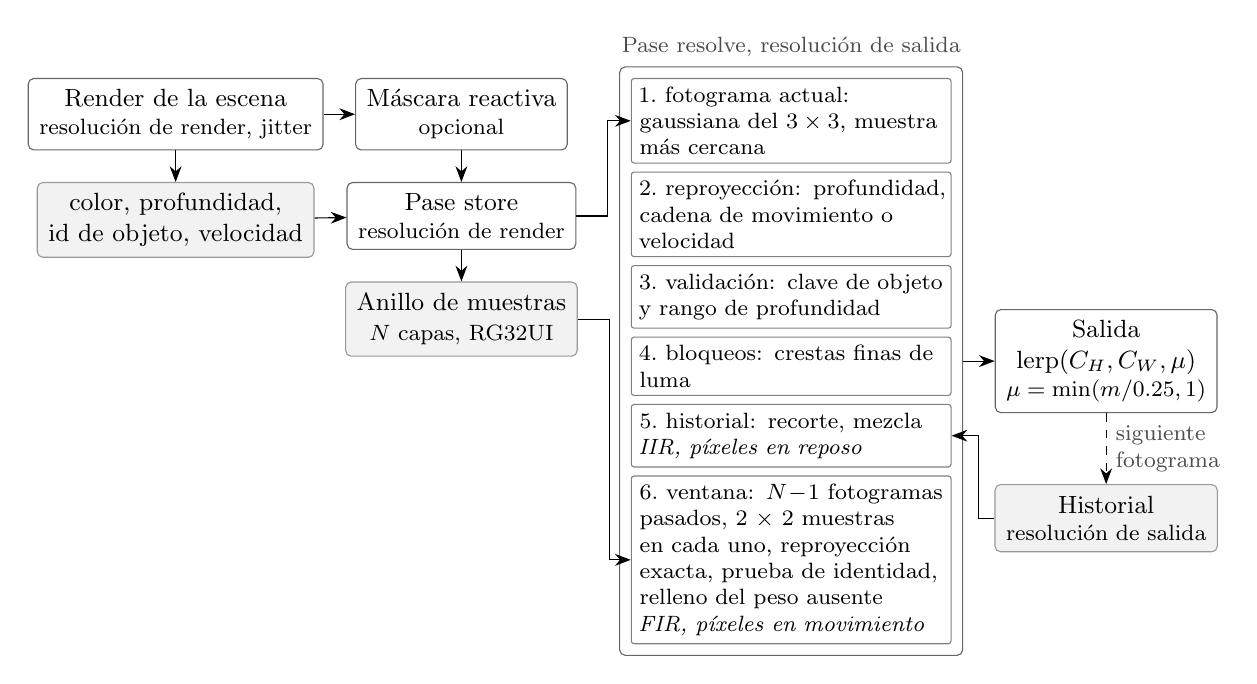
\begin{tikzpicture}[
  font=\small, >={Stealth[length=2mm]},
  box/.style={draw=black!60, rounded corners=2pt, align=center, inner sep=4pt, fill=white},
  data/.style={draw=black!40, fill=black!5, rounded corners=2pt, align=center, inner sep=4pt},
  stage/.style={draw=black!50, rounded corners=1pt, align=left, inner sep=3pt, fill=white, font=\footnotesize, text width=3.85cm},
  lbl/.style={font=\footnotesize, text=black!70}]
\node[box] (render) {Render de la escena\\[-1pt]{\footnotesize resolución de render, jitter}};
\node[data, below=4mm of render] (gbuf) {color, profundidad,\\id de objeto, velocidad};
\node[box, right=4mm of render] (react) {Máscara reactiva\\[-1pt]{\footnotesize opcional}};
\node[box, below=4mm of react] (store) {Pase store\\[-1pt]{\footnotesize resolución de render}};
\node[data, below=4mm of store] (ring) {Anillo de muestras\\{\footnotesize $N$ capas, RG32UI}};
\node[stage, right=8mm of react.north east, anchor=north west] (s1) {1.\ fotograma actual: gaussiana del $3\times3$, muestra más cercana};
\node[stage, below=1mm of s1] (s2) {2.\ reproyección: profundidad, cadena de movimiento o velocidad};
\node[stage, below=1mm of s2] (s3) {3.\ validación: clave de objeto y rango de profundidad};
\node[stage, below=1mm of s3] (s4) {4.\ bloqueos: crestas finas de luma};
\node[stage, below=1mm of s4] (s5) {5.\ historial: recorte, mezcla\\\textit{IIR, píxeles en reposo}};
\node[stage, below=1mm of s5] (s6) {6.\ ventana: $N\!-\!1$ fotogramas pasados, $2\times2$ muestras en cada uno, reproyección exacta, prueba de identidad, relleno del peso ausente\\\textit{FIR, píxeles en movimiento}};
\node[draw=black!60, rounded corners=2pt, inner sep=4pt, fit=(s1)(s6)] (resolve) {};
\node[lbl, above=0mm of resolve.north] {Pase resolve, resolución de salida};
\node[box, right=4mm of resolve] (out) {Salida\\$\mathrm{lerp}(C_H, C_W, \mu)$\\[-1pt]{\footnotesize $\mu=\min(m/0.25,1)$}};
\node[data, below=9mm of out] (hist) {Historial\\[-1pt]{\footnotesize resolución de salida}};
\draw[->] (render) -- (react);
\draw[->] (render) -- (gbuf);
\draw[->] (react) -- (store);
\draw[->] (gbuf) -- (store);
\draw[->] (store) -- (ring);
\draw[->] (ring.east) -- ++(4mm,0) |- (s6.west);
\draw[->] (store.east) -- ++(4mm,0) |- (s1.west);
\draw[->] (resolve) -- (out);
\draw[->, dashed] (out) -- node[lbl, right, align=left] {siguiente\\fotograma} (hist);
\draw[->] (hist.west) -- ++(-2mm,0) |- (s5.east);
\end{tikzpicture}
\caption{HWTAA en cada fotograma. El pase store escribe las muestras del fotograma en una capa del anillo. El resolve se ejecuta una vez por píxel de salida: los pasos 1 a 4 para todos los píxeles, el paso 5 para los que se mueven menos de $0.25$ píxeles de salida por fotograma, el paso 6 para los que se mueven algo, y la salida mezcla el historial $C_H$ y la ventana $C_W$ según el movimiento $m$.}
\label{fig:pipeline}
\end{figure}

HWTAA se ejecuta como dos pases de cómputo después de la geometría opaca y transparente (\cref{fig:pipeline}). El renderizador proporciona, a resolución de render y con un jitter de Halton$(2,3)$~\cite{halton1964}: color HDR lineal, profundidad, un identificador de recurso por píxel que da una clave de objeto estable y el movimiento del objeto, y un búfer de velocidad para las mallas deformadas. El \emph{pase store} empaqueta las muestras del fotograma en una capa de un búfer en anillo de $N$ capas. El \emph{pase resolve} reconstruye cada píxel de salida. Siempre reconstruye el fotograma actual en el centro del píxel y reproyecta y valida su historial. Para un píxel en reposo recorta y mezcla el historial como hace el TAA (\cref{sec:history}). Para un píxel en movimiento reúne del anillo las muestras de los $N-1$ fotogramas anteriores (\cref{sec:window}). La salida es
\begin{equation}
C = (1-\mu)\, C_H + \mu\, C_W, \qquad \mu = \min\!\left(\frac{m}{m_0}, 1\right), \quad m_0 = 0.25,
\label{eq:mix}
\end{equation}
donde $m$ es el movimiento de la superficie más cercana del píxel, en píxeles de salida por fotograma, $C_H$ la estimación del historial y $C_W$ la de la ventana. Los píxeles con $\mu = 1$ omiten el muestreo, el recorte y la mezcla del historial; los píxeles con $\mu=0$ omiten la ventana. La salida se escribe como historial del fotograma siguiente.

\subsection{Anillo de muestras}
\label{sec:ring}

Cada texel del anillo guarda una muestra de render en dos palabras de 32 bits. La \emph{palabra de información} guarda una clave de objeto de 16 bits (0 es el fondo) y los bits en media precisión de la profundidad de vista inversa $z = 1/d$. El bit de signo del valor en media precisión, siempre positivo, marca las muestras de objetos que no son estáticos, y su bit de mantisa más bajo, un cambio del 0.1\,\% en $z$, marca las muestras cubiertas por superficies transparentes. La \emph{palabra de color} guarda el color con el mapeo tonal $c/(1+\max(c))$, codificado en raíz cuadrada con 8 bits por canal, y la mediana de la luma con mapeo tonal de la vecindad $3\times3$ de la muestra, también en 8 bits. En nuestras escenas esta disposición igualó a un color en coma flotante de 16 bits con una diferencia de 0.02\,dB, mientras que canales de 6 bits perdieron de 0.2 a 0.3\,dB. Se guarda la profundidad inversa porque, con proyección en perspectiva, la profundidad NDC es afín en ella, lo que convierte la reproyección de la \cref{sec:window} en un único producto por una matriz, y porque el fondo en el infinito es simplemente $z=0$.

El anillo cuesta $8N$ bytes por texel de render. Su longitud en cada modo y su memoria se dan en la \cref{sec:cost}; cuando el presupuesto de memoria de la GPU no admite $N$ capas, la ventana se acorta, y por debajo de 4 capas se desactiva y el método se queda con su historial.

\subsection{Fotograma actual y reproyección}
\label{sec:current}

El fotograma actual se reconstruye en el centro $\vect p$ del píxel de salida a partir de las $3\times3$ muestras de render que lo rodean:
\begin{equation}
C_0(\vect p) = \frac{\sum_i w_i\, c_i}{\sum_i w_i}, \qquad w_i = e^{-k\,\|\vect x_i - \vect p\|^2}, \quad k = 4,
\label{eq:current}
\end{equation}
donde $\vect x_i$ es la posición con jitter de la muestra $i$ en píxeles de salida. El mayor peso, $w_{\max}$, mide lo bien que este fotograma cubre el píxel y es su parte en la mezcla del historial. La muestra con la mayor profundidad inversa del $3\times3$, la más cercana, representa al píxel en la reproyección, de modo que las siluetas siguen al primer plano. Su posición en el mundo se lleva al fotograma anterior solo con la cámara para los objetos estáticos, con la cadena de movimiento del objeto (el producto de sus transformaciones de objeto a mundo de ambos fotogramas) para los objetos que se mueven rígidamente, y con el búfer de velocidad para las mallas deformadas. Los pases resolve y store trabajan sobre grupos de $8\times8$ píxeles que cargan una sola vez en memoria compartida los texels de render que necesitan.

\subsection{Camino del historial}
\label{sec:history}

Para los píxeles en reposo, HWTAA es un TAA con tres cambios respecto al diseño habitual.

\paragraph{Validación por identidad.} En lugar de detectar la desoclusión por el color, el historial es válido cuando las $2\times2$ muestras anteriores alrededor de la posición reproyectada, leídas de la capa anterior del anillo, contienen la clave de objeto del píxel y la profundidad inversa esperada está dentro de su rango de profundidades (con un margen del 2\,\%). Una superficie estática delante de todas ellas también es válida: no pudo estar oculta, simplemente las muestras anteriores no la captaron, como ocurre con los cables y la transparencia estocástica.

\paragraph{Recorte y confianza.} El historial, muestreado con un filtro Catmull-Rom de cinco lecturas~\cite{jimenez2016filmic}, se recorta hacia la media de la caja de varianza~\cite{salvi2016taa} del $3\times3$ en YCoCg con mapeo tonal. La semianchura de la caja es una desviación típica, o $0.75$ para los objetos marcados como de sombreado volátil. Un historial recortado pierde confianza según el cuadrado de la razón de recorte. El canal alfa del historial guarda su confianza $n$, una suma de pesos de muestras, y la mezcla es
\begin{equation}
n' = \min(n + w_{\max},\; n_{\max}(m)), \qquad C_H = \mathrm{lerp}(H, C_0, w_{\max}/n'),
\end{equation}
con $n_{\max}(m) = \max(n_{\max}/(1+0.5\,m), 1)$: cada remuestreo emborrona el historial, así que su confianza se limita cuando el píxel se mueve. $n_{\max}$ vale $8\,s^{-2}$, acotado a $[8,32]$, para una escala de render $s$, y 256 cuando la escena está en reposo (nada se ha movido); el ciclo de jitter es en general de $8\,s^{-2}$ fases y de 64 en reposo, de modo que una imagen quieta sigue convergiendo. Las medias se toman en color lineal, que es el espacio de la referencia, y las mezclas se desplazan hacia el espacio con mapeo tonal a medida que el píxel se mueve, donde si no las muestras brillantes aisladas dejarían estela.

\paragraph{Bloqueos.} Un detalle fino es una cresta de luma (todos los vecinos que difieren más de un 5\,\% del centro están a un mismo lado de él) que ningún cuadrado de $2\times2$ que contenga el centro explica. Donde se encuentra uno, se crea un bloqueo; mientras vive, el historial no se recorta. Un bloqueo muere cuando la luma mediana del $3\times3$ cambia más de un factor 1.25 respecto a su valor al crearse, lo que es insensible al propio detalle (como mucho tres de nueve muestras) y sigue a cualquier cambio de sombreado que cubra la vecindad, como una sombra en movimiento. No vive ningún bloqueo sobre un borde geométrico, definido como un $3\times3$ cuyas profundidades inversas abarcan más de un 2\,\%; el fondo por sí solo no es un borde, así que las estrellas conservan sus bloqueos. Los bloqueos se evalúan en todos los píxeles, también en los que se mueven, de modo que sobreviven al movimiento y están listos cuando el píxel se detiene.

\paragraph{Separación de frecuencias.} Cuando la escala de render es como mucho 0.6 y la escena está en reposo, la caja del $3\times3$ a resolución de render no puede validar las frecuencias por encima del límite de Nyquist del render, y recortar todo el historial elimina el detalle que se acumuló más allá de él. Entonces el historial se separa en una banda baja, la media de cuatro lecturas bilineales en las diagonales a $0.5\,(s^{-1}-1)$ píxeles de salida por eje, que se recorta, y una banda alta, que se conserva dentro de dos semianchuras de la caja. Esto ganó 0.59\,dB en una escena estática a mitad de resolución.

\subsection{Ventana de muestras}
\label{sec:window}

Para un píxel en movimiento, la estimación de la ventana es
\begin{equation}
C_W(\vect p) = \frac{\frac{1}{1-r}\sum_{i} w_i c_i \;+\; \sum_{k=1}^{N-1} \sum_{j\in S_k} v_j\, \omega_j\, c_j \;+\; \omega_{\mathrm{aus}}\, \bar c_{\mathrm{otras}}}{\frac{1}{1-r}\sum_i w_i \;+\; \sum_{k=1}^{N-1}\sum_{j\in S_k} v_j\, \omega_j \;+\; \omega_{\mathrm{aus}}},
\label{eq:window}
\end{equation}
donde los primeros términos son el $3\times3$ actual de la \cref{eq:current}, $S_k$ son las cuatro muestras del anillo del fotograma $t-k$ más próximas a donde estaba entonces la superficie del píxel, $v_j\in\{0,1\}$ es la prueba de visibilidad, $\omega_j$ el peso de la muestra $j$ en su posición en el fotograma actual, $r$ el valor reactivo de la \cref{sec:reactive} y el último término el relleno del peso ausente de la \cref{sec:missing}.

\paragraph{Dónde buscar.} Para el fotograma $t-k$, la superficie más cercana del píxel se proyecta con la cámara de ese fotograma, a través de la cadena de movimiento del objeto para ese fotograma si se mueve rígidamente, y con $k$ veces la velocidad actual si se deforma. Las cuatro muestras del anillo más próximas a esa posición se leen en un solo viaje a memoria: cada texel es una única lectura de 64 bits con todo lo que necesitan la prueba y el peso.

\paragraph{Reproyección exacta por muestra.} Una muestra del propio objeto en movimiento del píxel se mueve con él: su desplazamiento respecto al centro del píxel ahora es su desplazamiento respecto a la posición de la superficie entonces. Cualquier otra muestra se mueve según su propia profundidad y ambas cámaras, lo que es exacto para las superficies estáticas. Con proyección en perspectiva, la profundidad NDC es afín en la profundidad inversa $z$, y la posición NDC de la muestra es afín en sus coordenadas de texel $(u,v)$ y su jitter. Toda la cadena, desde el texel, el jitter y la profundidad inversa del fotograma $t-k$, pasando por el espacio del mundo, hasta el espacio de recorte del fotograma actual y finalmente a píxeles de salida escalados a unidades de peso, es por tanto una sola matriz:
\begin{equation}
\begin{pmatrix} x\\ y\\ \cdot\\ w \end{pmatrix} = \mathbf{W}_k \begin{pmatrix} u\\ v\\ z\\ 1 \end{pmatrix},
\qquad \vect g_j = \left(\frac{x}{w}, \frac{y}{w}\right) - \vect g(\vect p), \qquad \omega_j = 2^{-\|\vect g_j\|^2},
\label{eq:reproject}
\end{equation}
donde $\mathbf{W}_k = \mathbf{U}\,\mathbf{P}_t\,\mathbf{P}_{t-k}^{-1}\,\mathbf{T}_k$, $\mathbf{T}_k$ lleva un texel y su profundidad inversa a NDC en el fotograma $t-k$, $\mathbf{P}$ son las matrices de vista y proyección sin jitter, y $\mathbf{U}$ lleva NDC a píxeles de salida multiplicados por $\sqrt{k\log_2 e}$, de modo que $2^{-\|\vect g\|^2}$ es igual a la gaussiana de la \cref{eq:current}. $\mathbf{W}_k$ se calcula en la CPU, una vez por fotograma para cada fotograma de la ventana. Como las cuatro muestras de un fotograma comparten sus términos de texel, una muestra cuesta tres multiplicaciones-sumas, una división y el peso. Las muestras a más de un píxel de salida del centro en algún eje se descartan antes de calcular el peso; su peso sería inferior a $e^{-4}$.

\paragraph{Visibilidad por identidad.} Una muestra cuenta ($v_j=1$) cuando la muestra actual en su nueva posición, que está en el $3\times3$ del píxel y ya está en memoria compartida, pertenece al mismo objeto y es estática, o pertenece al propio objeto en movimiento del píxel. La oclusión y la desoclusión se derivan de esta única prueba, sin acotado de color: en nuestras escenas, acotar cada muestra pasada al $3\times3$ actual borraba los detalles finos. Una excepción cubre los primeros planos finos: cuando el objeto más cercano ocupa como mucho dos de las nueve muestras actuales, como ocurre con un cable, sus muestras pasadas estáticas también cuentan donde están delante de la superficie actual, porque las muestras actuales simplemente no lo captaron.

\paragraph{Sombreado que se mueve por su cuenta.} El movimiento de los objetos no describe las sombras en movimiento, los materiales animados ni las superficies transparentes dibujadas sobre la escena opaca. Para los objetos marcados como volátiles, para los píxeles cuyo valor reactivo supera $0.1$ y para las muestras pasadas marcadas como transparentes, un fotograma pasado se descarta cuando la luma mediana guardada con su muestra más próxima difiere de la actual más de un factor 1.25. Los objetos volátiles usan la ventana incluso en reposo, donde el historial dejaría estela detrás de una sombra en movimiento, si la escala de render es al menos 0.6 y la ventana tiene al menos 8 fotogramas.

\paragraph{Mallas deformadas.} Las mallas deformadas no tienen cadena de movimiento; sus posiciones pasadas se extrapolan a partir de la velocidad actual, que se aparta de la trayectoria real cuando el movimiento cambia. Su ventana se limita a 6 fotogramas, valor elegido con un disco ondulante.

\paragraph{Traspaso de confianza.} Un píxel que usa solo la ventana no calcula su historial, pero sí lo escribe: la estimación de la ventana pasa a ser el historial, y el peso total de la ventana, en unidades de fotogramas actuales, pasa a ser su confianza. Cuando el píxel se detiene, el historial parte de las muestras acumuladas en la ventana.

\subsection{Relleno del peso ausente}
\label{sec:missing}

La ventana lee cada fotograma pasado donde estaba la superficie más cercana del píxel. En el borde de un objeto en movimiento, las demás superficies se movieron de otra manera: estaban ocultas detrás de él, o se quedaron atrás al pasar la cámara junto a ellas. Sus muestras pasadas están en otro lugar, mientras que las de la superficie más cercana están todas ahí, así que la ventana arrastra el borde hacia la superficie más cercana, lo que se ve como un fantasma fino. HWTAA restablece el equilibrio: para cada fotograma pasado en el que no contó ninguna muestra de otra superficie, cada muestra de otra superficie que no contó añade a $\omega_{\mathrm{aus}}$ el peso que habría tenido en la posición de la superficie más cercana. El color asignado a ese peso, $\bar c_{\mathrm{otras}}$, es la media gaussiana, en el fotograma actual, de las muestras de otras superficies del $3\times3$, con una gaussiana más ancha ($k=1$) porque a mitad de resolución la más próxima puede estar a dos píxeles. Esto se aplica a los píxeles de objetos en movimiento y a los bordes geométricos. En el fotograma siguiente a que un píxel quede descubierto, el relleno reduce allí el error un \nGhostCutNat\,\% a resolución nativa y un \nGhostCutQ\,\% en modo Calidad (\cref{fig:ghost}).

\subsection{Máscara reactiva}
\label{sec:reactive}

Las superficies transparentes se dibujan sobre la escena opaca y no tienen movimiento propio. HWTAA construye su máscara él mismo a partir del color antes y después del pase transparente:
\begin{equation}
r = \min\!\big(4\,\max_{c}|T(c_{\mathrm{después}}) - T(c_{\mathrm{antes}})|,\; 1\big), \qquad T(c) = \frac{c}{1+\max(c)}.
\end{equation}
Mide lo que las superficies transparentes le hicieron al texel, así que las superficies con mezcla alfa y las aditivas cuentan igual, y una superficie que no cambia nada, como la parte vacía de un sprite, no cuenta. En la ventana, los fotogramas pasados cuentan $(1-r)$ veces lo que el actual; la confianza del historial y los bloqueos se escalan por $(1-r)$, y las muestras con $r > 0.1$ se marcan como transparentes en el anillo.

\section{Implementación}
\label{sec:implementation}

HWTAA está implementado en \emph{eevee-game}, el renderizador en tiempo real del motor de juegos UPBGE~\cite{upbge}, como shaders de cómputo GLSL: un pase store a resolución de render, un pase resolve a resolución de salida y, cuando la escena tiene superficies transparentes, los dos despachos de la máscara reactiva alrededor del pase transparente. Los dos pases principales usan grupos de $8\times8$. El resolve carga en memoria compartida los texels de render de la huella de su grupo, hasta $10\times10$, emitiendo todas las lecturas antes del primer uso para que sus latencias se solapen, y lee el $3\times3$ de cada píxel con desplazamientos constantes desde una sola dirección.

El resolve está dimensionado para 64 registros vectoriales en AMD GCN, lo que permite cuatro frentes de onda por SIMD; lo comprobamos con el compilador ACO de Mesa~\cite{mesa}. Varias decisiones se derivan de ese presupuesto: el color que usa el relleno del peso ausente se calcula en el paso~1 y se aparca en memoria compartida, el bucle de fotogramas pasados no se especializa por tipo de píxel, y las cuatro muestras de un fotograma se procesan con una función desenrollada en lugar de un bucle interno. En la CPU se construyen, para cada fotograma de la ventana, la matriz $\mathbf{W}_k$ de la \cref{eq:reproject}, la vista-proyección anterior, el jitter y la capa del anillo, y para cada objeto en movimiento su cadena de movimiento a lo largo de la ventana.

Cada modo de calidad tiene una escala de render y una longitud de ventana: Nativo ($s=1$, $N=8$), Ultra Calidad ($1/1.3$, 14), Calidad ($1/1.5$, 14), Equilibrado ($1/1.7$, 14) y Rendimiento ($1/2$, 12). Mientras la cámara se mueve y la escala es al menos 0.6, el ciclo de jitter es igual a la longitud de la ventana, de modo que cada ventana contiene el mismo patrón subpíxel. Equilibrado y Rendimiento usan ventanas no más largas que la de Calidad para no costar nunca más que Calidad, cuyos usuarios tienen las GPU más rápidas. Las aplicaciones pueden fijar el presupuesto de memoria y la longitud de la ventana.

\section{Evaluación}
\label{sec:evaluation}

\subsection{Configuración}

\paragraph{Banco de pruebas.} La evaluación ejecuta los shaders de producción mediante un contexto OpenGL~4.3 (Mesa llvmpipe, en una máquina sin GPU), sobre escenas renderizadas analíticamente en la CPU. Solo se sustituyen las declaraciones de recursos propias del motor por declaraciones GLSL estándar; la parte de CPU del módulo (matrices, cadenas de movimiento, jitter, gestión del anillo) está portada a Python. La salida es de $192\times108$ píxeles; la referencia de cada fotograma es un filtro de caja supermuestreado $6\times6$ (36 muestras por píxel); se renderizan 60 fotogramas y se miden los fotogramas 30 a 59. Las imágenes se comparan tras el mapeo tonal $c/(1+c)$. Todos los números, tablas y figuras de esta sección los producen los scripts del banco de pruebas que acompañan al artículo; las mediciones de diseño citadas en la \cref{sec:method} proceden de la versión de desarrollo del mismo banco.

\paragraph{Escenas.} Todas las escenas comparten una pared con un degradado suave, líneas diagonales de 0.35 píxeles de ancho cada 9 píxeles, una franja de cuadros de 2 píxeles, un disco teñido y luces puntuales HDR de 0.6 píxeles de ancho, y, delante, un disco a rayas que se mueve 1.7 píxeles por fotograma. La cámara se desplaza $(0.37, 0.13)$ píxeles por fotograma. \emph{paneo} es esta escena base; \emph{cables} añade dos cables oscuros de 0.4 píxeles de ancho, más cerca de la cámara; \emph{suelo} añade un plano de suelo con textura de cuadros y líneas finas en perspectiva, y un cielo con estrellas HDR en el infinito; \emph{suelo rápido} desplaza la escena del suelo a 4 píxeles por fotograma; \emph{deformación} hace ondular el disco a rayas de forma no rígida; \emph{humo} añade un panel de vidrio, una partícula de humo a la deriva con densidad animada y una chispa aditiva; \emph{ruido} multiplica cada muestra por un factor aleatorio de desviación típica 0.3, como haría un sombreado estocástico; \emph{zoom +} y \emph{zoom $-$} cambian el campo de visión un 3\,\% por fotograma; \emph{paneo-parada} y \emph{paneo-reposo} detienen la cámara en el fotograma 30, con el disco aún en movimiento en la primera y quieto en la segunda, donde el renderizador pasa a reposo; \emph{sombra} mueve una franja de sombra sobre una escena estática; y \emph{estática} no mueve nada.

\paragraph{Métricas.} Damos el PSNR, \FLIP{}~\cite{andersson2020flip} y el SSIM~\cite{wang2004ssim} de los fotogramas codificados en sRGB, y una métrica de parpadeo: la diferencia absoluta media entre el cambio de un fotograma al siguiente de la salida y el de la referencia, por 1000. Los errores por región (error absoluto medio por 1000) aíslan los píxeles que el disco en movimiento descubrió en los últimos 8 fotogramas, los cables, el cielo, el disco deformado y la estela del humo.

\paragraph{Referencias de comparación.} El TAA de referencia sigue el diseño de producción de Karis~\cite{karis2014taa}: jitter de Halton$(2,3)$ en 8 fotogramas, movimiento de la muestra más cercana del $3\times3$ con vectores de movimiento exactos por píxel, historial Catmull-Rom, recorte por varianza ($\gamma=1$) en YCoCg con mapeo tonal y un factor de mezcla de 0.1. Se ejecuta a resolución nativa, con el fotograma actual reconstruido a partir de la propia muestra del píxel (TAA\textsubscript{p}) o de una gaussiana del $3\times3$ que aproxima el filtro de Blackman-Harris de Karis (TAA\textsubscript{G}); en cada escena comparamos con el mejor de los dos. \emph{Sin AA} toma una muestra sin jitter por píxel.

\subsection{Calidad}

\begin{table}[t]
\centering
\setlength{\tabcolsep}{3.5pt}
\caption{Resumen de las \nNumScenes{} escenas. \emph{Píx.\ render}: píxeles renderizados por píxel de salida. PSNR en dB. \emph{Victorias}: escenas en las que el PSNR supera al mejor TAA de referencia. Los modos de escalado se comparan con el TAA a resolución nativa, que renderiza de 1.7 a 4 veces más píxeles.}
\label{tab:summary}
\small
\begin{tabular}{lrrrrrrr}
\toprule
M\'etodo & P\'ix. render & PSNR mov. $\uparrow$ & PSNR total $\uparrow$ & \FLIP $\downarrow$ & SSIM $\uparrow$ & Parpadeo $\downarrow$ & Victorias \\
\midrule
Sin AA & 100\,\% & 27.14 & 27.62 & 0.0467 & 0.777 & 24.3 &  \\
TAA\textsubscript{p} & 100\,\% & 29.68 & 30.04 & 0.0487 & 0.859 & 11.9 &  \\
TAA\textsubscript{G} & 100\,\% & 29.38 & 29.45 & 0.0409 & 0.825 & 12.8 &  \\
\midrule
HWTAA Nativo & 100\,\% & 35.56 & 35.81 & 0.0236 & 0.965 & 7.1 & 13/13 \\
HWTAA U.\,Cal. & 59\,\% & 33.58 & 33.98 & 0.0309 & 0.943 & 8.8 & 13/13 \\
HWTAA Calidad & 44\,\% & 32.54 & 32.90 & 0.0340 & 0.931 & 9.8 & 13/13 \\
HWTAA Equil. & 35\,\% & 31.25 & 31.85 & 0.0398 & 0.908 & 11.1 & 12/13 \\
HWTAA Rend. & 25\,\% & 30.40 & 31.07 & 0.0419 & 0.891 & 12.0 & 10/13 \\
\bottomrule
\end{tabular}

\end{table}

\begin{table}[t]
\centering
\caption{PSNR (dB) por escena; el mejor valor de cada fila en negrita.}
\label{tab:quality}
\small
\begin{tabular}{lrrrrrrrr}
\toprule
 & \multicolumn{3}{c}{} & \multicolumn{5}{c}{HWTAA} \\
\cmidrule(lr){5-9}
Escena & Sin AA & TAA\textsubscript{p} & TAA\textsubscript{G} & Nativo & U.\,Cal. & Calidad & Equil. & Rend. \\
\midrule
\multicolumn{9}{l}{\textit{Movimiento}} \\
\quad paneo & 26.28 & 28.91 & 28.53 & \textbf{36.02} & 33.42 & 32.46 & 30.87 & 30.51 \\
\quad cables & 25.75 & 28.61 & 28.31 & \textbf{34.55} & 32.38 & 31.55 & 30.18 & 29.78 \\
\quad suelo & 26.49 & 29.22 & 28.78 & \textbf{34.87} & 33.29 & 32.48 & 31.29 & 30.34 \\
\quad suelo r\'apido & 27.74 & 29.47 & 28.48 & \textbf{33.46} & 31.04 & 30.16 & 29.33 & 28.37 \\
\quad deformaci\'on & 26.27 & 28.91 & 28.53 & \textbf{35.93} & 33.30 & 32.35 & 30.79 & 30.34 \\
\quad humo & 26.71 & 29.19 & 28.75 & \textbf{35.87} & 33.30 & 32.38 & 30.94 & 30.49 \\
\quad ruido & 22.69 & 28.40 & 28.31 & \textbf{32.58} & 31.28 & 30.21 & 28.92 & 27.95 \\
\quad zoom + & 33.78 & 33.77 & 33.81 & \textbf{41.47} & 40.21 & 38.75 & 37.46 & 35.52 \\
\quad zoom $-$ & 28.59 & 30.63 & 30.89 & \textbf{35.30} & 34.01 & 32.49 & 31.45 & 30.31 \\
\quad\textit{media} & \textit{27.14} & \textit{29.68} & \textit{29.38} & \textit{35.56} & \textit{33.58} & \textit{32.54} & \textit{31.25} & \textit{30.40} \\
\multicolumn{9}{l}{\textit{Movimiento que se detiene}} \\
\quad paneo-parada & 28.03 & 30.93 & 30.09 & \textbf{36.83} & 35.09 & 33.49 & 33.67 & 32.72 \\
\quad paneo-reposo & 28.14 & 31.17 & 30.33 & \textbf{37.85} & 36.07 & 34.60 & 34.04 & 33.35 \\
\quad\textit{media} & \textit{28.08} & \textit{31.05} & \textit{30.21} & \textit{37.34} & \textit{35.58} & \textit{34.05} & \textit{33.85} & \textit{33.03} \\
\multicolumn{9}{l}{\textit{C\'amara fija}} \\
\quad sombra & 29.46 & 29.66 & 28.41 & \textbf{34.49} & 32.67 & 31.74 & 30.64 & 29.84 \\
\quad est\'atica & 29.11 & 31.63 & 29.59 & \textbf{36.36} & 35.68 & 35.05 & 34.43 & 34.36 \\
\quad\textit{media} & \textit{29.29} & \textit{30.64} & \textit{29.00} & \textit{35.42} & \textit{34.18} & \textit{33.39} & \textit{32.54} & \textit{32.10} \\
\midrule
Todas las escenas, media & 27.62 & 30.04 & 29.45 & 35.81 & 33.98 & 32.90 & 31.85 & 31.07 \\
\bottomrule
\end{tabular}

\end{table}

Las \cref{tab:summary,tab:quality} recogen los resultados. A resolución nativa, HWTAA alcanza \nPsnrAllNat{}\,dB frente a \nPsnrAllBestTAA{}\,dB del mejor TAA en cada escena, una ganancia de \nGainAllNat{}\,dB de media (\nGainMotionNat{}\,dB en movimiento) y de al menos \nWorstGainNat{}\,dB en todas las escenas; el parpadeo baja de \nFlickerTAApt{} a \nFlickerNat{} y \FLIP{} de \nFlipTAAg{} a \nFlipNat{}. Los modos de escalado cambian calidad por coste de render en orden: Ultra Calidad y Calidad superan al TAA en todas las escenas renderizando el 59\,\% y el 44\,\% de sus píxeles, Equilibrado en \nWinsB{} de \nNumScenes{} y Rendimiento, con el 25\,\%, en \nWinsP{} de \nNumScenes{}. Rendimiento pierde frente al TAA en \emph{suelo rápido} ($\nWorstGainP$\,dB), \emph{zoom $-$} y \emph{ruido}: con un cuarto de las muestras, un paneo de 4 píxeles por fotograma deja demasiado pocas muestras por píxel en una ventana de 12 fotogramas, y el ruido por muestra se promedia sobre menos muestras de las que guarda el historial del TAA.

\begin{figure}[t]
\centering
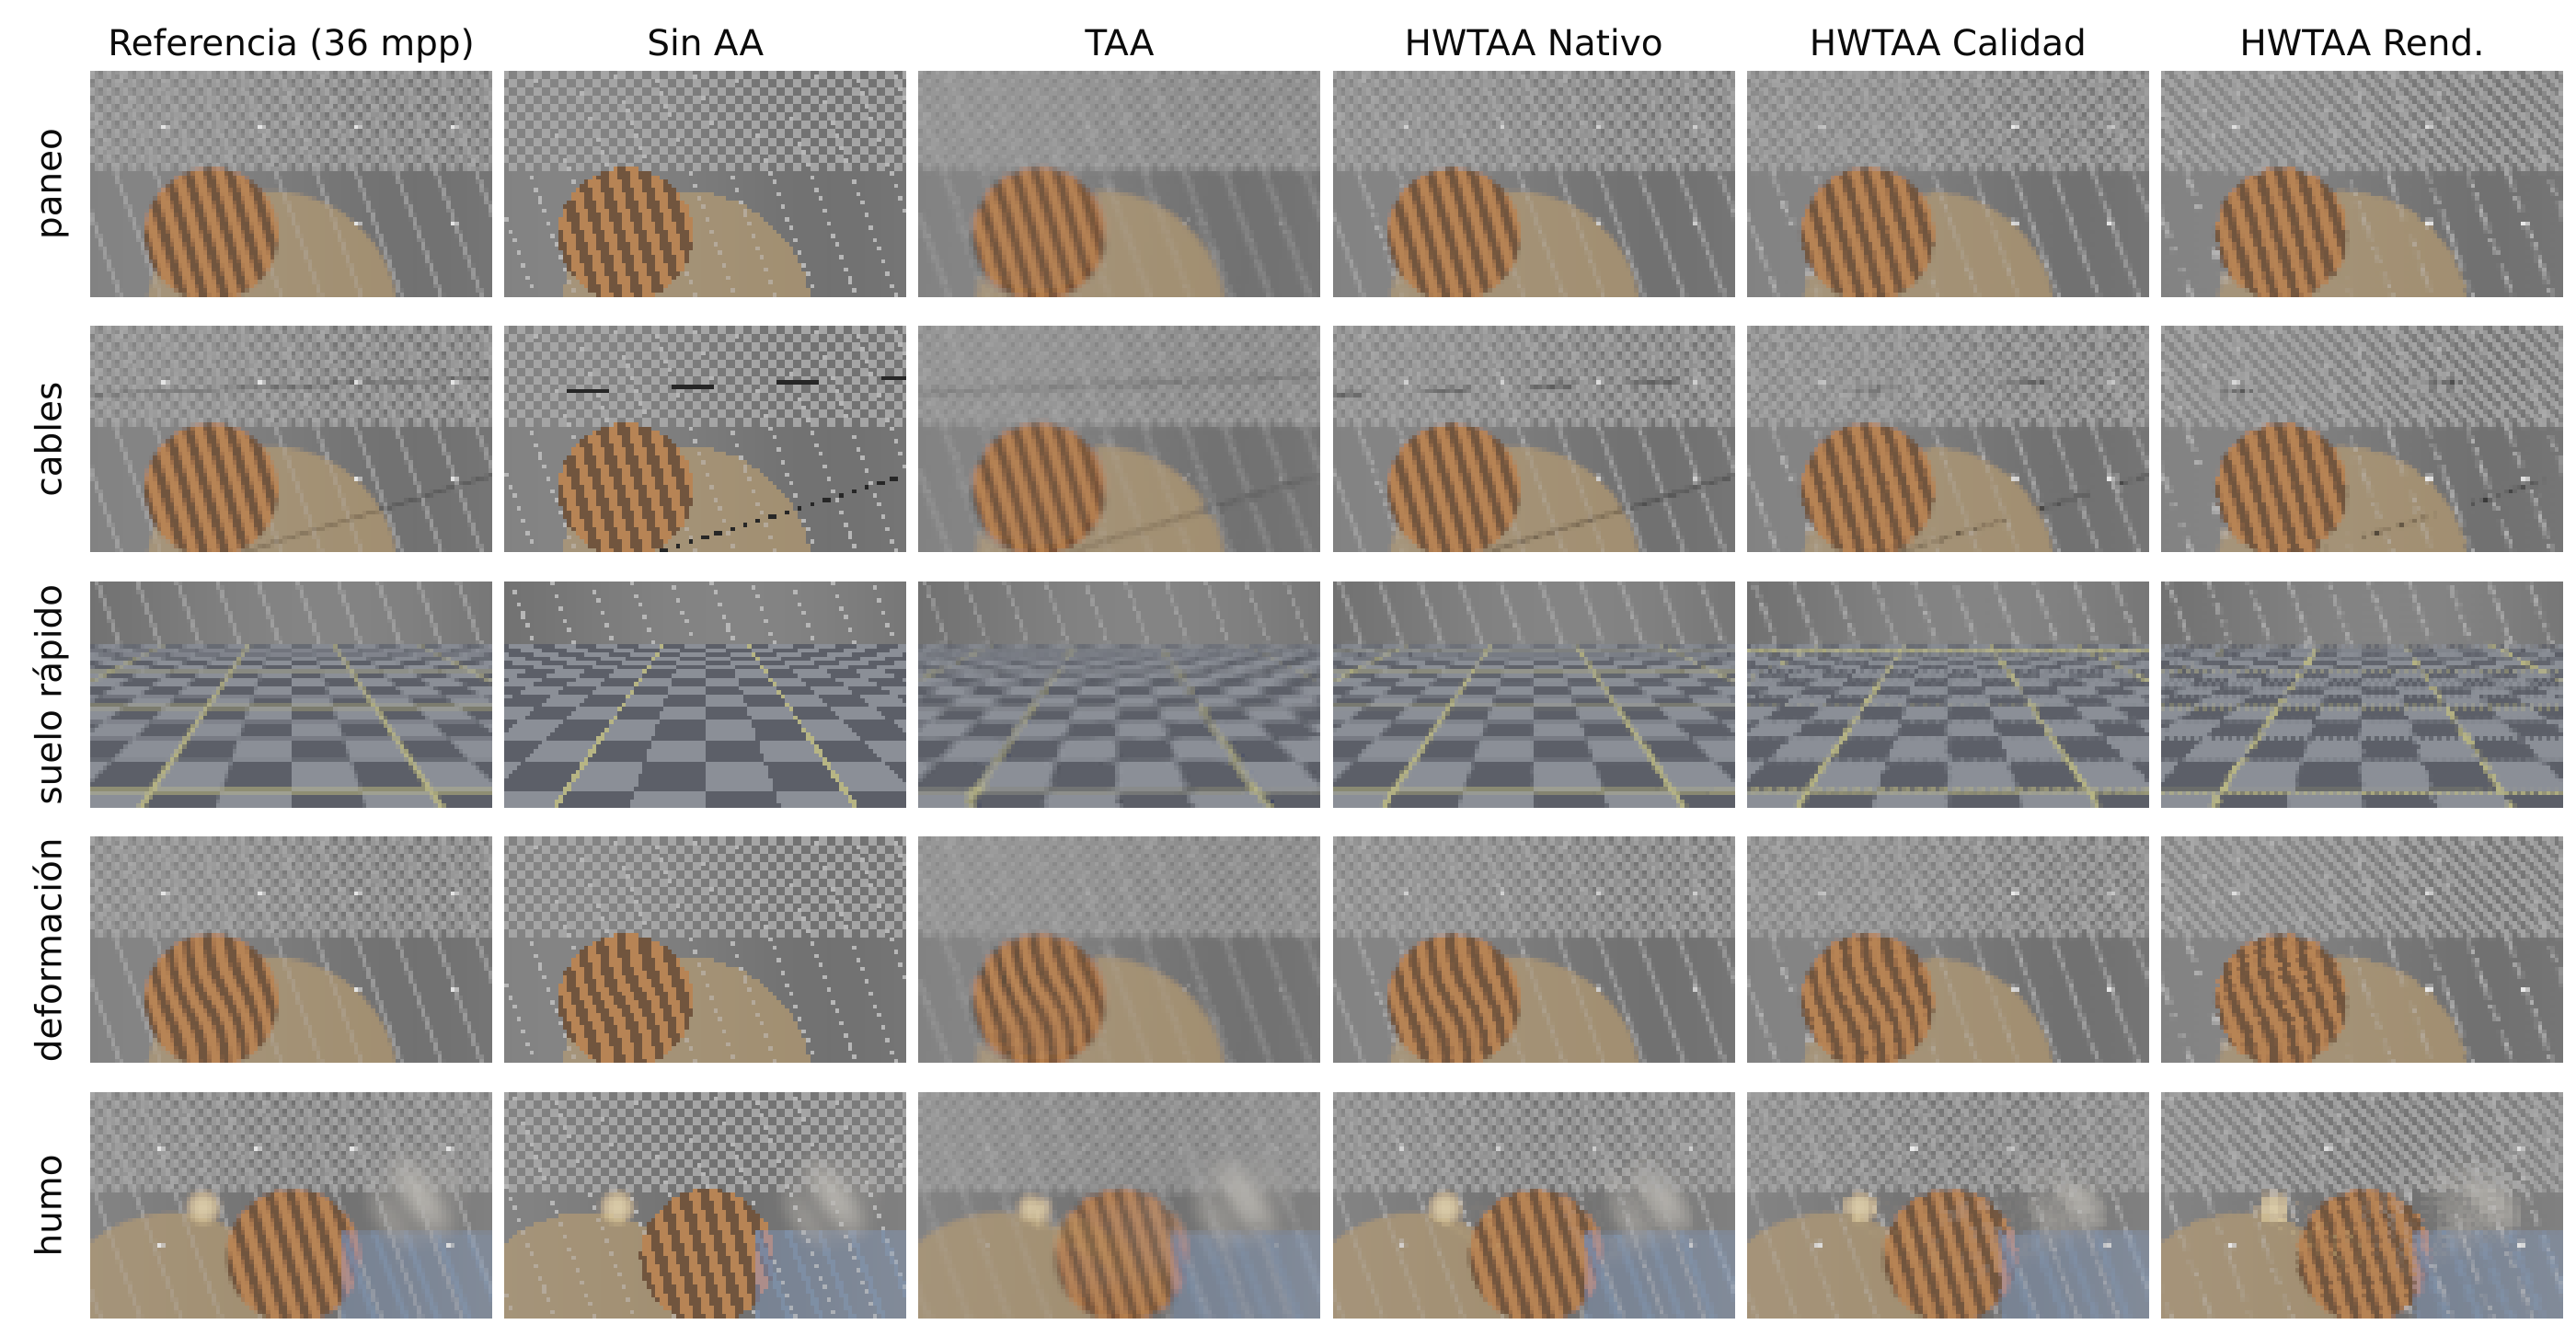
\includegraphics[width=\textwidth]{crops.png}
\caption{Fotograma 45 de cinco escenas, recortes de $96\times54$ ampliados por vecino más próximo. El TAA emborrona los cuadros de 2 píxeles y las líneas en movimiento y pierde la mayor parte de los cables; HWTAA Nativo los conserva. Los modos de escalado renderizan el 44\,\% (Calidad) y el 25\,\% (Rendimiento) de los píxeles: los cables se rompen en trazos y el disco deformado muestra su patrón de muestreo en Rendimiento.}
\label{fig:crops}
\end{figure}

La \cref{fig:crops} muestra la diferencia en movimiento. El historial del TAA, remuestreado en cada fotograma, ha perdido los cuadros, las líneas y la mayor parte de los cables; la ventana, que nunca remuestrea, los conserva. Con escalas de render bajas la ventana tiene demasiado pocas muestras para los detalles subpíxel: los cables se vuelven discontinuos en Calidad y Rendimiento, y el disco deformado, cuya ventana es de 6 fotogramas, muestra su patrón de muestreo.

\subsection{Longitud de la ventana}

\begin{figure}[t]
\centering
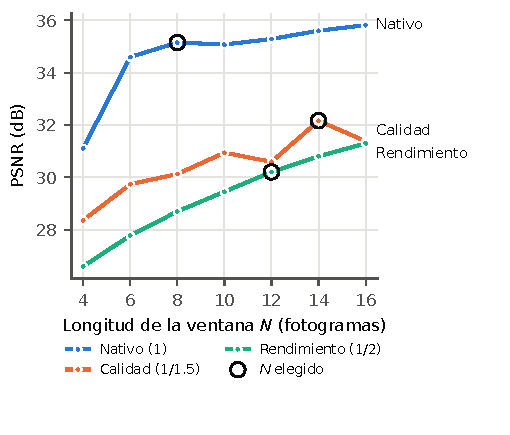
\includegraphics[width=0.62\textwidth]{window.pdf}
\caption{PSNR frente a la longitud de la ventana $N$, media de \emph{paneo}, \emph{cables} y \emph{suelo}, por escala de render. Los círculos marcan la longitud con la que se distribuye cada modo. Con escala de render $1/1.5$, la longitud de la ventana es también el ciclo de jitter en movimiento, y los ciclos de 12 y 16 fases cubren el píxel peor que el de 14.}
\label{fig:window}
\end{figure}

La \cref{fig:window} muestra el efecto de la longitud de la ventana. A resolución nativa la ganancia se satura tras 6 a 8 fotogramas; 14 a 16 fotogramas ganan otros 0.5 a 0.7\,dB, pero cada fotograma cuesta unos \nMsPerFrameHd{}\,ms a 1080p para los píxeles en movimiento. Al escalar, cada fotograma añade muestras que le faltan al píxel de salida; a mitad de resolución el PSNR sigue subiendo hasta 16 fotogramas. Las longitudes elegidas son una decisión de coste.

\subsection{Desoclusión}

\begin{figure}[t]
\centering
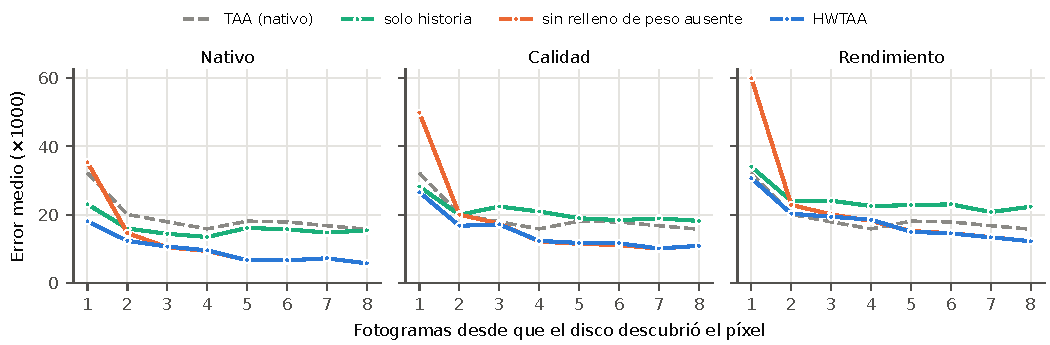
\includegraphics[width=\textwidth]{ghost.pdf}
\caption{Error medio ($\times1000$) en los píxeles que descubrió el disco en movimiento de \emph{paneo}, según los fotogramas transcurridos desde que quedaron descubiertos. Sin el relleno del peso ausente, la ventana arrastra el borde del disco al primer fotograma tras descubrirse; el historial solo sigue emborronado en los fotogramas siguientes.}
\label{fig:ghost}
\end{figure}

La \cref{fig:ghost} sigue los píxeles que descubre el disco en movimiento. En el primer fotograma tras descubrirse, la ventana sola es peor que el historial, porque la superficie descubierta no tiene allí muestras pasadas y las muestras del disco arrastran el borde; el relleno del peso ausente lleva el error por debajo del del historial (\nGhostHwNatOne{} frente a \nGhostNoFillNatOne{} sin relleno y \nGhostHistNatOne{} con solo el historial, a resolución nativa). A partir del segundo fotograma, la ventana tiene muestras reales de la superficie descubierta y su error es de media un \nGhostVsHistNat\,\% menor que el del historial a resolución nativa y un \nGhostVsHistQ\,\% menor en Calidad.

\subsection{Ablaciones}

\begin{table}[t]
\centering
\caption{Ablaciones: cada variante elimina un componente. Los cambios de PSNR son medias sobre las escenas en las que actúa el componente: solo historial, paneo, cables, suelo, suelo rápido, deformación y humo; solo ventana, paneo-reposo y estática; relleno del peso ausente, las mismas que solo historial salvo humo; bloqueos, paneo-reposo, estática, suelo y suelo rápido; las demás, la escena de su región afectada. En las demás escenas del conjunto de ablación el cambio es como mucho de \nAblNoMissingFillRest{}\,dB, salvo en la variante de solo historial, que también cambia paneo-reposo en $\nAblHistoryOnlyPausestopNat$\,dB. Las dos últimas columnas dan el cambio relativo del error o del parpadeo en la región afectada.}
\label{tab:ablation}
\footnotesize\setlength{\tabcolsep}{3.5pt}
\begin{tabular}{lrrlrr}
\toprule
Variante & $\Delta$ Nativo & $\Delta$ Calidad & \multicolumn{3}{c}{Regi\'on afectada} \\
\cmidrule(lr){4-6}
 & dB & dB & & Nativo & Calidad \\
\midrule
Solo historial (sin ventana) & $-5.65$ & $-4.41$ & descubierto (paneo) & $+50$\,\% & $+31$\,\% \\
Solo ventana (sin historia) & $-0.30$ & $-0.03$ & parpadeo (est\'atica) & $+161$\,\% & $+147$\,\% \\
Sin relleno del peso ausente & $-0.35$ & $-0.37$ & descubierto (paneo) & $+27$\,\% & $+25$\,\% \\
Sin bloqueos de luma & $-2.56$ & $-2.88$ & cielo (suelo r\'apido) & $+25$\,\% & $+3$\,\% \\
Sin regla de primer plano fino & $-0.22$ & $-0.16$ & cables (cables) & $+12$\,\% & $+12$\,\% \\
Sin ventana en mallas deformadas & $-0.59$ & $-0.72$ & disco deformado (deformaci\'on) & $+62$\,\% & $+104$\,\% \\
Sin m\'ascara reactiva & $-2.27$ & $-1.44$ & estela de humo (humo) & $+133$\,\% & $+140$\,\% \\
\bottomrule
\end{tabular}

\end{table}

La \cref{tab:ablation} elimina los componentes de uno en uno, a resolución nativa y en modo Calidad. Sin la ventana, el PSNR de las escenas en movimiento cambia en $\nAblHistoryOnlyNat$\,dB a resolución nativa y en $\nAblHistoryOnlyQ$\,dB en modo Calidad: la ventana es la contribución principal. Sin el historial, el PSNR apenas cambia de media, pero en la escena estática el PSNR cambia en $\nAblWindowOnlyStaticNat$\,dB y el parpadeo en un $\nAblWindowOnlyStaticNatFlicker$\,\%, porque la ventana deja de converger tras $N$ fotogramas, y el resolve cuesta más: en un píxel en reposo, el camino del historial cuesta el \nHistShareNat\,\% del camino de la ventana a resolución nativa y el \nHistShareQ\,\% en modo Calidad. Justo después de que la cámara se detiene (\emph{paneo-reposo}), la ventana sola obtiene $\nAblWindowOnlyPausestopNat$\,dB frente al híbrido, cuyo historial aún no ha convergido; volvemos sobre ello en la \cref{sec:limitations}. Los bloqueos son esenciales para los detalles finos en reposo ($\nAblNoLocksStaticNat$\,dB en \emph{estática} sin ellos). Sin la máscara reactiva, el error de la estela del humo crece un \nAblNoReactiveTgtNatAbs\,\% a resolución nativa; sin la ventana en las mallas deformadas, el error del disco deformado crece un \nAblNoDeformedWindowTgtNatAbs\,\% a resolución nativa y un \nAblNoDeformedWindowTgtQAbs\,\% en modo Calidad. La regla del primer plano fino y el relleno del peso ausente tienen efectos menores pero consistentes allí donde se aplican.

\subsection{Coste y memoria}
\label{sec:cost}

\begin{table}[t]
\centering
\caption{Coste y memoria. HWTAA: tiempo estimado en una RX~590 (clase GTX~1060) con los píxeles en reposo y con toda la pantalla en movimiento, el peor caso; memoria en MB con el anillo, el historial, los bloqueos, los identificadores de objeto y la máscara reactiva. \textsuperscript{a}FSR~2.2: medido por AMD en una RX~590~\cite{amd2023fsr2}. \textsuperscript{b}FSR~3.1: cifras de AMD para una RX~5700~XT~\cite{amd2024fsr3,amd2025fsr31manual}, una GPU más rápida, solo como referencia.}
\label{tab:cost}
\small
\begin{tabular}{llrrrrrrrr}
\toprule
 & & & \multicolumn{2}{c}{HWTAA (ms)} & \multicolumn{2}{c}{FSR (ms)} & \multicolumn{3}{c}{Memoria (MB)} \\
\cmidrule(lr){4-5}\cmidrule(lr){6-7}\cmidrule(lr){8-10}
Salida & Modo & $N$ & Quieto & En mov. & 2.2\textsuperscript{a} & 3.1\textsuperscript{b} & HWTAA & 2.2 & 3.1 \\
\midrule
1080p & Nativo & 8 & 0.8 & 1.4 & -- & 1.7 & 189 & -- & -- \\
 & Ultra Calidad & 14 & 0.7 & 2.0 & -- & -- & 188 & -- & -- \\
 & Calidad & 14 & 0.6 & 2.0 & 1.3 & 1.2 & 151 & 115 & 75 \\
 & Equilibrado & 14 & 0.6 & 2.0 & 1.2 & -- & 127 & 105 & 65 \\
 & Rendimiento & 12 & 0.6 & 1.8 & 1.1 & 1.0 & 95 & 101 & 61 \\
\midrule
1440p & Nativo & 8 & 1.4 & 2.5 & -- & 3.0 & 335 & -- & -- \\
 & Ultra Calidad & 14 & 1.2 & 3.6 & -- & -- & 333 & -- & -- \\
 & Calidad & 14 & 1.1 & 3.6 & 2.3 & 2.0 & 269 & 207 & 134 \\
 & Equilibrado & 14 & 1.1 & 3.6 & 2.1 & -- & 226 & 189 & 118 \\
 & Rendimiento & 12 & 1.1 & 3.1 & 1.9 & 1.7 & 169 & 172 & 101 \\
\midrule
4K & Nativo & 8 & 3.2 & 5.5 & -- & 6.5 & 755 & -- & -- \\
 & Ultra Calidad & 14 & 2.6 & 8.2 & -- & -- & 750 & -- & -- \\
 & Calidad & 14 & 2.6 & 8.1 & 5.4 & 4.4 & 605 & 448 & 292 \\
 & Equilibrado & 14 & 2.5 & 8.0 & 4.9 & -- & 508 & 407 & 256 \\
 & Rendimiento & 12 & 2.4 & 7.0 & 4.4 & 3.7 & 379 & 376 & 226 \\
\bottomrule
\end{tabular}

\end{table}

No dispusimos de GPU para este trabajo, así que el coste se estima de forma estática. El compilador ACO da el inverso del rendimiento de cada shader por frente de onda en AMD Polaris; lo convertimos en tiempo en una RX~590 (36 unidades de cómputo a 1.545\,GHz) con un único factor, que lleva los propios shaders de FSR~2.2, compilados del mismo modo, a los 1.3\,ms medidos por AMD a 1080p en modo Calidad en esa GPU~\cite{amd2023fsr2}. El pase store escala con los píxeles de render y el resolve con los de salida; los tiempos publicados de FSR~2.2 en la misma GPU escalan igual (1.78 y 4.15 veces el tiempo de 1080p a 1440p y 4K). Además, cada estimación tiene como mínimo el tiempo de su tráfico de memoria a 192\,GB/s, el ancho de banda de una GTX~1060; esto solo importa a resolución nativa, donde un píxel en reposo mueve unos 73 bytes. El banco de pruebas incluye un script que mide ambos pases con consultas de tiempo de la GPU en hardware real.

La \cref{tab:cost} compara las estimaciones con FSR. En reposo, HWTAA cuesta aproximadamente la mitad que FSR~2.2 en los modos de escalado (\nMsStillQHd{} frente a 1.3\,ms a 1080p en Calidad). Con toda la pantalla en movimiento, el coste de la ventana crece con $N$, unos \nMsPerFrameHd{}\,ms por fotograma a 1080p, y HWTAA cuesta de 1.5 a 1.6 veces lo que FSR~2.2 (\nMsMovingQHd{} frente a 1.3\,ms a 1080p en Calidad, \nMsMovingQUhd{} frente a 5.4\,ms a 4K). A resolución nativa no hay modo de FSR~2.2 con el que comparar; el Native AA de FSR~3.1 tarda 1.7\,ms a 1080p en una GPU más rápida, frente a \nMsStillNatHd{} a \nMsMovingNatHd{}\,ms de HWTAA. La memoria la domina el anillo: en modo Calidad es 1.3 veces la de FSR~2.2 y 2 veces la de FSR~3.1; en modo Rendimiento es similar a la de FSR~2.2.

\section{Limitaciones y trabajo futuro}
\label{sec:limitations}

\paragraph{Evaluación.} Las escenas son sintéticas y pequeñas, y su referencia es analítica. Se diseñaron para aislar los casos que el TAA resuelve mal, así que sus medias exageran la ganancia en el contenido típico de un videojuego, donde gran parte de la pantalla está en reposo y ambos métodos convergen. Los tiempos son estimaciones del compilador, no mediciones; la calibración con FSR~2.2 los hace comparables con las cifras de AMD, pero el coste real depende de la GPU, el controlador y la escena. No medimos en el banco de pruebas la calidad de imagen de FSR, DLSS ni otros escaladores. Un estudio con contenido de videojuegos en hardware real, frente a estos métodos, es el siguiente paso natural.

\paragraph{Coste y memoria en movimiento.} La ventana cuesta unos \nMsPerFrameHd{}\,ms por fotograma de ventana a 1080p para los píxeles en movimiento, \nMsPerFrameUhd{}\,ms a 4K, lo que hace que un paneo a pantalla completa en 4K sea más caro que con FSR. Su anillo ocupa de 1.3 a 2 veces la memoria de FSR. Ambos se pueden ajustar con la longitud de la ventana y el presupuesto de memoria, a razón de unos 0.3\,dB por fotograma de ventana al escalar.

\paragraph{Escalas de render bajas.} Con un cuarto de los píxeles, una ventana de 12 fotogramas contiene tres muestras por píxel de salida; el movimiento rápido, el ruido fuerte por muestra y el zoom hacia fuera favorecen entonces la acumulación más larga del TAA.

\paragraph{Píxeles que se detienen.} Durante unos fotogramas después de que un píxel se detiene, su historial no ha convergido mientras que la ventana aún contiene $N$ muestras válidas (\emph{paneo-reposo} en la \cref{tab:ablation}). Mantener la ventana hasta que la confianza del historial alcance el peso de la ventana eliminaría este hueco.

\paragraph{Requisitos del motor.} El método necesita claves de objeto estables, el movimiento de los objetos en los últimos $N$ fotogramas y un búfer de velocidad para las mallas deformadas, que un motor de juegos tiene pero un posproceso inyectado en una aplicación arbitraria no. Las mallas deformadas extrapolan sus posiciones pasadas a partir de la velocidad actual, lo que limita su ventana a unos pocos fotogramas.

\section{Conclusión}

El TAA resume el pasado en una imagen y lo paga en cada fotograma en que un píxel se mueve. HWTAA guarda las propias muestras pasadas durante una ventana corta, lleva cada una de ellas una sola vez y de forma exacta al fotograma actual, decide su visibilidad por identidad, y conserva el historial recursivo solo donde mejor funciona, en los píxeles en reposo. En nuestras escenas esto mejora un TAA de calidad de producción en \nGainAllNat{}\,dB a resolución nativa y en \nGainAllQ{}\,dB escalando desde el 44\,\% de los píxeles, y mantiene nítidos en movimiento los cables, las líneas y la textura fina. El precio es la memoria del anillo y un coste en movimiento que crece con la ventana, ambos ajustables por la aplicación.

\section*{Uso de herramientas de IA}
El método lo desarrolló el autor con la ayuda de Claude (Anthropic), un modelo de IA, usado como asistente de programación e investigación: implementó y midió variantes bajo la dirección del autor, construyó el banco de pruebas y ayudó a redactar este manuscrito. El autor dirigió el trabajo, tomó las decisiones de diseño y es responsable del contenido. La herramienta de IA no figura como autora.

\section*{Código y datos}
Los shaders y el banco de pruebas, con los scripts que producen todas las tablas y figuras, están en el mismo repositorio que este artículo, bajo la Licencia Pública General de GNU versión 2 o posterior, como el motor UPBGE.

\bibliographystyle{unsrtnat}
\bibliography{../refs}

\end{document}
